\normalfalse \difficiletrue \tdifficilefalse
\correctionfalse

%\UPSTIidClasse{12} % 11 sup, 12 spé
%\newcommand{\UPSTIidClasse}{12}

\exer{Mouvement RT -- RSG  $\star\star$ \label{C2:09:09}}
\setcounter{question}{0}\UPSTIcompetence[2]{C2-09}
\index{Compétence C2-09}
\index{Principe fondamental de la dynamique}
\index{PFD}
\index{Mécanisme à 1 rotations, 1 translation et RSG}
\index{Culbuto}
\ifcorrection
\else
\marginnote{\textbf{Pas de corrigé pour cet exercice.}}
\fi

\ifprof
\else
Soit le mécanisme suivant. On a $\vect{IA}=R\vect{j_0}$ et $\vect{AB}=\lambda(t)\vect{i_1}$. De plus $R=\SI{15}{mm}$.
On fait l'hypothèse de roulement sans glissement au point $I$. De plus :
\begin{itemize}
\item $G_1$ désigne le centre d'inertie de \textbf{1} tel que $\vect{AG_1}=-\ell\vect{i_1}$, on note $m_1$ la masse de \textbf{1} et $\inertie{G_1}{1}=\matinertie{A_1}{B_1}{C_1}{0}{0}{0}{\bas{1}}$; 
\item $G_2=B$ désigne le centre d'inertie de \textbf{2}, on note $m_2$ la masse de \textbf{2} et $\inertie{G_2}{2}=\matinertie{A_2}{B_2}{C_2}{0}{0}{0}{\bas{2}}$.
\end{itemize}
Un ressort exerce une action mécanique entre les points $A$ et $B$. 
\begin{center}
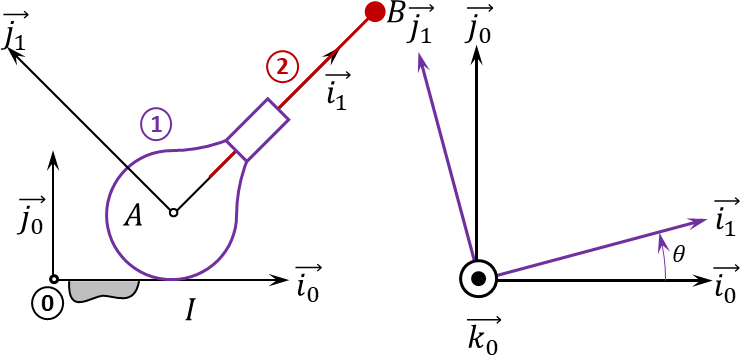
\includegraphics[width=\linewidth]{09_RT_RSG_01}
\end{center}
\fi

L'objectif est d'obtenir les lois de mouvement. 

\question{Appliquer le théorème de la résultante dynamique au solide \textbf{2}  en projection sur $\vect{i_1}$}
\ifprof
\else
\fi

\question{Appliquer le théorème du moment dynamique à l'ensemble \textbf{1+2} au point $I$ en projection sur $\vect{k_0}$.}
\ifprof
\else
\fi


\ifprof
\else
\begin{flushright}
\footnotesize{Corrigé  voir \ref{C2:09:09}.}
\end{flushright}%
\fi